\documentclass{article}

\usepackage[final]{project_nips_style}

% =========================
% Packages
% =========================
\usepackage[utf8]{inputenc}
\usepackage[T1]{fontenc}
\usepackage{hyperref}
\usepackage{url}
\usepackage{booktabs}
\usepackage{amsmath, amsfonts}
\usepackage{graphicx}
\graphicspath{{../../results/}}
\usepackage{microtype}
\usepackage[table]{xcolor}
\usepackage{colortbl}

% Grey/white row shading used by the strategy table (matches DL_Project_Report.pdf style)
\definecolor{tableGrey}{gray}{0.90}
\definecolor{headerGrey}{gray}{0.80}

% =========================
% Title Information
% =========================
\title{Freezing Strategies in Transfer Learning for Skin Lesion Classification\\
\large Deep Learning Project Report S26}

\author{%
  \begin{tabular}{cc}
    \textbf{Harsh Naik}                                 & \textbf{Avin Pathak} \\
    University of Bern                                  & University of Bern \\
    \texttt{harsh.nayak@students.unibe.ch}              & \texttt{avin.pathak@students.unibe.ch} \\[1.2ex]
    \textbf{Daksahaini Chellappah}                      & \textbf{Jasmin Injodikaran} \\
    University of Bern                                  & University of Bern \\
    \texttt{daksahaini.chellappah@students.unibe.ch}    & \texttt{jasmin.injodikaran@students.unibe.ch} \\
  \end{tabular}%
}

\begin{document}

\maketitle

\vspace{0.5em}

% ============================================================
\section{Introduction and Background}
% ============================================================

Transfer learning has become a key method in deep learning, allowing models
trained on large datasets to be efficiently adapted to new domains where data
is often limited. A central question in this process is how much of the
previously learned knowledge should be preserved, frozen, or fine-tuned when
moving to a different task~\cite{yosinski2014transferable}.

This project examines different strategies for freezing layers in transfer
learning applied to the classification of skin lesions, a task of clear
clinical importance, where labeled data are scarce and accurate predictions
can have direct diagnostic value~\cite{esteva2017dermatologist}. By
systematically testing various freezing configurations, we aim to better
understand the balance between preserving general visual representations and
adapting to task-specific features.

We take inspiration from an analogy in medical training: when a general
practitioner specializes in dermatology, they keep their foundational
understanding of medicine (such as anatomy and physiology) but develop new,
focused expertise. In a similar way, a pre-trained neural network retains
basic visual patterns like edges and textures that remain useful, while its
higher-level layers often need to be fine-tuned to capture the subtle
distinctions between different kinds of skin lesions.

\begin{quote}
\textit{``When adapting a pre-trained model to a new task, how much of its
previously learned knowledge should be retained?''}
\end{quote}

% ============================================================
\section{Method}
% ============================================================

We use the HAM10000 dataset (Human Against Machine with 10{,}000 training
images), accessible via Kaggle and TensorFlow
Datasets~\cite{tschandl2018ham10000}. Key dataset properties:

\begin{itemize}
  \item 10{,}015 dermoscopic images across 7 classes: melanoma (MEL),
  melanocytic nevi (NV), basal cell carcinoma (BCC), actinic keratosis
  (AKIEC), benign keratosis (BKL), dermatofibroma (DF), and vascular lesions
  (VASC).
  \item Significant class imbalance (NV dominates with $\sim$67\% of samples).
  \item Standard train/validation/test splits are applied with stratified
  sampling.
  \item Preprocessing: resize to $224\times224$, ImageNet normalization,
  augmentation (flip, rotation, color jitter).
\end{itemize}

Due to class imbalance, we apply a class-weighted loss during training and
report balanced accuracy and macro-averaged AUC as primary metrics.

\subsection{Model Architecture}

We use EfficientNet-B0 pre-trained on ImageNet as our primary backbone, due
to its favorable accuracy--efficiency trade-off and widespread use in medical
imaging benchmarks. ResNet18 is used for cross-architecture validation in a
subset of experiments, allowing us to separate strategy effects from
architecture effects.

We compare three freezing strategies:

\begin{table}[h]
\centering
\caption{Three transfer-learning strategies evaluated on each backbone.}
\label{tab:strategies}
\begin{tabular}{|p{0.18\linewidth}|p{0.38\linewidth}|p{0.34\linewidth}|}
\hline
\textbf{Strategy} & \textbf{Description} & \textbf{Expected Behaviour} \\
\hline
\rowcolor{tableGrey}
S1 -- From Scratch &
All weights randomly initialised; full network trained on HAM10000 &
Weakest performance; lower bound baseline due to limited data \\
\hline
S2 -- Full Freeze &
All pre-trained weights frozen; only the classification head is trained &
Fast training; may underfit if ImageNet features are insufficient \\
\hline
\rowcolor{tableGrey}
S3 -- Gradual Unfreeze &
Start with frozen backbone; progressively unfreeze layer blocks every few
epochs &
Best generalisation; balances retained knowledge with task-specific
adaptation \\
\hline
\end{tabular}
\end{table}

\subsection{Training Setup}

In this project, we train a neural network to classify images of skin
lesions using the HAM10000 dataset. This dataset contains just over $10{,}000$
images divided into seven different classes (MEL, NV, BCC, AKIEC, BKL, DF,
VASC). One important challenge is that the dataset is heavily imbalanced ---
melanocytic nevi (NV) alone account for roughly $67\%$ of the samples. To
handle this, we split the dataset into training, validation, and test sets
($80\%$, $10\%$, and $10\%$) using stratified sampling, which keeps the same
class distribution in each split. This ensures that the model is evaluated
fairly across all classes.

Before training, the images are preprocessed. First, all images are resized
to $224\times224$ pixels so they can be used as input to the neural network.
Next, the images are normalised using the standard ImageNet mean and
standard deviation, since both backbones (EfficientNet-B0 and ResNet18) are
pre-trained on ImageNet. During training only, we apply data augmentation in
the form of random horizontal flips and random rotations of up to $\pm
10^{\circ}$. This helps the model generalise better by exposing it to mild
geometric variation in the data.

To train the model, we use the cross-entropy loss function, which measures
how wrong the model's predictions are. Because the dataset is imbalanced, we
use class weights computed on the training split with sklearn's
\texttt{balanced} scheme so that mistakes on rare classes (DF, VASC, AKIEC)
are penalised more than mistakes on common ones (NV). This helps the model
learn all classes more equally.

We use the Adam optimiser to update the model during training. Adam is a
commonly used optimisation method that automatically adjusts how fast each
parameter learns. It works well for deep learning tasks and converges
quickly. The initial learning rate is set to $10^{-3}$ while only the
classification head is trainable. For the gradual-unfreeze strategy (S3),
the optimiser is rebuilt at a smaller learning rate of $10^{-4}$ after each
unfreezing event, so newly trainable feature blocks are updated more gently
and the pre-trained features are not disturbed.

Finally, we define several hyperparameters, which are settings chosen before
training. These include a batch size of $32$ (how many images are processed
at once), $5$ training epochs per strategy, and an unfreeze interval of $1$
epoch for S3 (one feature block is unfrozen at the start of every epoch
after the first). Rather than using early stopping, we save the best
checkpoint by validation accuracy after every epoch, so the final test
evaluation always uses the strongest model observed during training.

\subsection{Implementation Details}

The code is organised as a small package with namespace imports
(\texttt{data/}, \texttt{models/}, \texttt{evaluation/}); all entry points
(\texttt{train\_s1.py}, \texttt{train\_s2.py}, \texttt{train\_s3.py},
\texttt{main.py}) are thin wrappers around
\texttt{models.train.run\_strategy}, which loads data, builds the requested
model, trains, evaluates on the held-out test split, and persists training
curves, confusion matrices, and a metrics JSON. Optimiser parameter groups
are built with \texttt{filter(lambda p: p.requires\_grad,
model.parameters())} so frozen parameters never receive gradients; the
optimiser is rebuilt after each S3 unfreezing event so new trainable
parameters are picked up. The S3 unfreeze logic is backbone-specific: for
EfficientNet, blocks of \texttt{model.features.children()} are unfrozen
top-down; for ResNet18, \texttt{layer4} $\to$ \texttt{layer1} via
\texttt{unfreeze\_resnet\_block}.

% ============================================================
\section{Results}
% ============================================================

Table~\ref{tab:results-enet} reports the test-set metrics for the three
freezing strategies on the EfficientNet-B0 backbone. The ranking is monotone
and unambiguous: S3 $>$ S2 $\gg$ S1.

\begin{table}[h]
\centering
\caption{Test-set results on HAM10000 (EfficientNet-B0, 5 epochs).
Higher is better for all metrics.}
\label{tab:results-enet}
\begin{tabular}{lccc}
\toprule
Strategy & Balanced Acc. & Macro $F_1$ & Macro AUC \\
\midrule
S1 -- From Scratch       & 0.375 & 0.225 & 0.811 \\
S2 -- Full Freeze        & 0.639 & 0.472 & \textbf{0.916} \\
S3 -- Gradual Unfreeze   & \textbf{0.661} & \textbf{0.495} & 0.915 \\
\bottomrule
\end{tabular}
\end{table}

\begin{figure}[h]
\centering

\includegraphics[width=0.78\linewidth]{strategy_comparison.png}
\caption{Cross-strategy comparison on the HAM10000 test split
(EfficientNet-B0). The S1$\to$S2 jump dominates; S3 adds a small further gain
on balanced accuracy and macro $F_1$.}
\label{fig:strategy-comparison}
\end{figure}

\textbf{Why the model performs as it does.} S1 collapses on the rare classes
(per-class $F_1$ of $0.00$ for both BCC and DF), confirming that
$\sim$8k training images are insufficient to train $\sim$5M parameters from
scratch~\cite{tajbakhsh2016convolutional}. S2 lifts balanced accuracy by
$+26.4$ points by simply re-using ImageNet edges/textures and learning a 7-way
linear head on top of them --- the largest single jump in the table. S3 adds
a further $+2.2$ points on balanced accuracy and $+2.3$ on macro~$F_1$ by
allowing the higher feature blocks to specialise toward dermoscopic texture
while a reduced learning rate ($10^{-4}$) protects the lower
blocks~\cite{yosinski2014transferable}.

\textbf{Comparison to baseline / cross-architecture validation.} Treating S1
as the from-scratch baseline, S2 and S3 both more than double its macro
$F_1$. The S3-vs-S2 comparison, however, is \emph{architecture-dependent}:
on EfficientNet-B0, best validation accuracy was \emph{higher} for S2
(67.3\%) than for S3 (64.9\%), even though S3 narrowly wins on the
class-imbalance-aware test metrics in Table~\ref{tab:results-enet}; on
ResNet18, S3 (73.0\% best val acc) clearly outperformed S2 (65.8\%). We
attribute the EfficientNet inversion to the very short 5-epoch budget --- S3
only finishes unfreezing toward the end of training and so has little time
to converge --- and the ResNet result to the fact that ResNet18 benefits
more from deeper adaptation to dermoscopic texture than the already-compact
EfficientNet-B0 features do.

\textbf{Failure cases.} The dominant residual error mode for both S2 and S3
is the rare-class$\to$NV confusion driven by the class prior ($\sim$2/3 of
training samples are NV). Class-weighted loss substantially mitigates but
does not eliminate this; per-class $F_1$ for DF remains the lowest at $0.18$
(S2) / $0.31$ (S3), reflecting only a few hundred DF training images.

% ============================================================
\section{Conclusion}
% ============================================================

\textbf{What was achieved.} A clean, reproducible comparison of three
transfer-learning regimes on HAM10000 with two ImageNet backbones
(EfficientNet-B0, ResNet18), with class-imbalance-aware training and
evaluation throughout.

\textbf{Key findings.} (1) Re-using pre-trained features is essential ---
S1$\to$S2 alone closes most of the gap. (2) Gradual unfreezing did
\emph{not} consistently outperform full freezing across architectures. The
best validation accuracies were:
\begin{itemize}
  \item EfficientNet-B0 -- S3 (Gradual Unfreeze): 64.9\%
  \item ResNet18 -- S2 (Full Freeze): 65.8\%
  \item ResNet18 -- S3 (Gradual Unfreeze): \textbf{73.0\%} (best overall).
\end{itemize}
On EfficientNet-B0, S2 reached a slightly higher validation accuracy than S3
(67.3\% vs.\ 64.9\%), most likely because the 5-epoch budget leaves S3 with
too few epochs after unfreezing to converge. On ResNet18 the gap reverses
and S3 clearly wins. (3) Putting (1) and (2) together: gradual unfreezing
appears more beneficial for architectures that need stronger adaptation to
the target domain (ResNet18 here), while a strong frozen backbone with a
trained head can be sufficient --- and even preferable under tight compute
budgets --- for architectures whose ImageNet features already transfer well
(EfficientNet-B0).

\textbf{Limitations.} Only 5 epochs per run, no learning-rate schedule, no
hyper-parameter sweep, single random seed, and no test-time
augmentation/ensembling. The macro AUC of S3 is marginally below S2, hinting
that gradual unfreezing reorganises the probability mass without strictly
improving ranking quality.

\textbf{Possible improvements.} Longer training with cosine annealing;
per-block discriminative learning rates rather than a single $10^{-4}$
post-unfreeze rate; oversampling rare classes (DF, VASC) in addition to
weighted loss; and a stronger augmentation pipeline (colour jitter,
dermoscopic-specific transforms) to attack the rare-class confusion
identified in the failure analysis. Parameter-efficient
adapters~\cite{hu2021lora} and lottery-ticket-style sparse
fine-tuning~\cite{frankle2019lottery,morcos2019oneticket} are natural next
steps for the partial-re-use regime.

{\small
\bibliographystyle{plainnat}
\bibliography{references}
}

% ============================================================
\appendix
% ============================================================

\newpage
\section{Appendix}

\subsection{Per-class $F_1$ on the test split (EfficientNet-B0)}

\begin{table}[h]
\centering
\begin{tabular}{lccccccc}
\toprule
Strategy & MEL & NV & BCC & AKIEC & BKL & DF & VASC \\
\midrule
S1 & 0.339 & 0.700 & 0.000 & 0.159 & 0.118 & 0.000 & 0.260 \\
S2 & 0.415 & 0.790 & 0.510 & 0.492 & 0.543 & 0.176 & 0.377 \\
S3 & 0.414 & 0.770 & 0.541 & 0.530 & 0.544 & 0.313 & 0.351 \\
\bottomrule
\end{tabular}
\end{table}

\subsection{Confusion matrices (EfficientNet-B0)}

The diagonal of the S1 confusion matrix is dominated by NV (the prior class)
with whole rows for BCC, DF and VASC routed away from their true class.
S2 already balances the diagonal substantially, and S3 further reduces the
rare-class$\to$NV leakage discussed in \S3.

\begin{figure}[h]
\centering
\begin{minipage}[t]{0.32\linewidth}
  \centering
  
\includegraphics[width=\linewidth]{S1_confusion_matrix.png}
  \subcaption*{S1 -- From Scratch}
\end{minipage}\hfill
\begin{minipage}[t]{0.32\linewidth}
  \centering
  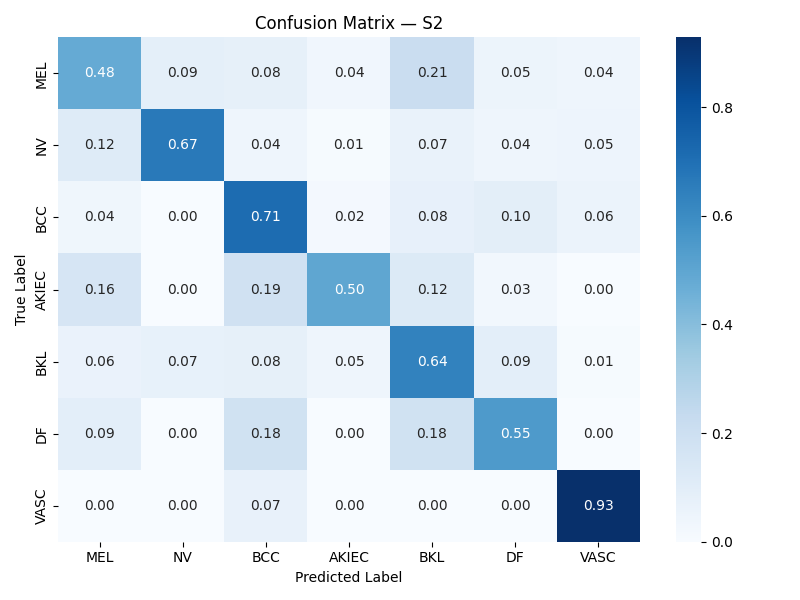
\includegraphics[width=\linewidth]{S2_confusion_matrix.png}
  \subcaption*{S2 -- Full Freeze}
\end{minipage}\hfill
\begin{minipage}[t]{0.32\linewidth}
  \centering
  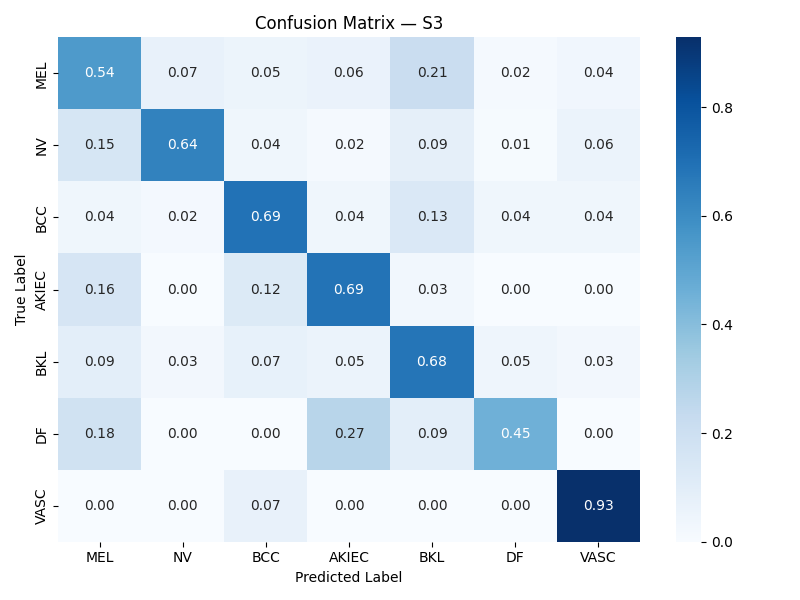
\includegraphics[width=\linewidth]{S3_confusion_matrix.png}
  \subcaption*{S3 -- Gradual Unfreeze}
\end{minipage}
\caption{Row-normalised confusion matrices on the HAM10000 test split
(EfficientNet-B0).}
\label{fig:confusion-matrices}
\end{figure}

\subsection{Training curves (EfficientNet-B0)}

The S3 curve shows the characteristic accuracy bumps after each unfreezing
event, while S1 lags far below both pre-trained variants throughout
training.

\begin{figure}[h]
\centering
\begin{minipage}[t]{0.32\linewidth}
  \centering
  
\includegraphics[width=\linewidth]{S1_training_curves.png}
  \subcaption*{S1}
\end{minipage}\hfill
\begin{minipage}[t]{0.32\linewidth}
  \centering
  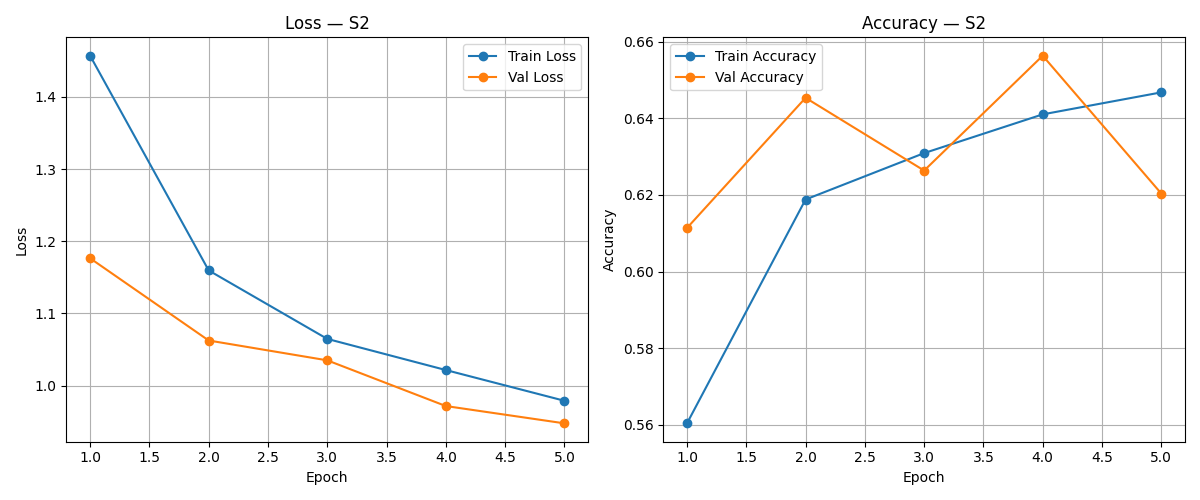
\includegraphics[width=\linewidth]{S2_training_curves.png}
  \subcaption*{S2}
\end{minipage}\hfill
\begin{minipage}[t]{0.32\linewidth}
  \centering
  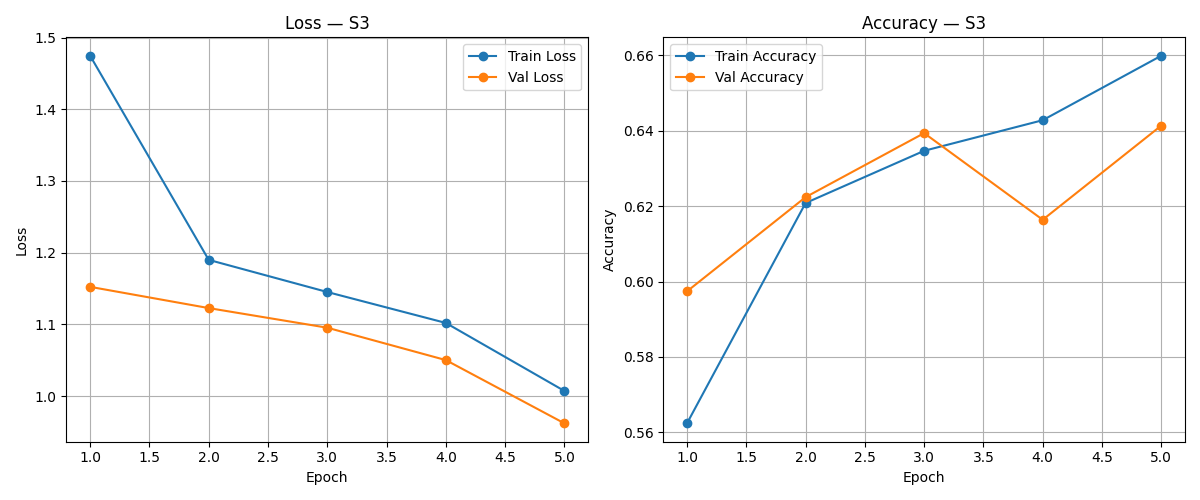
\includegraphics[width=\linewidth]{S3_training_curves.png}
  \subcaption*{S3}
\end{minipage}
\caption{Per-strategy train/val loss and accuracy curves over the 5-epoch
budget (EfficientNet-B0).}
\label{fig:training-curves}
\end{figure}

\subsection{Reproducibility}

All experiments are launched from the project root with the
\texttt{skin-lesion} conda environment. Splits are exported once via
\texttt{python data/export\_splits.py}; the three strategies are then
reproduced with \texttt{python train\_s1.py}, \texttt{train\_s2.py},
\texttt{train\_s3.py}, or end-to-end with \texttt{python main.py}. Each run
writes \texttt{results/\{S1,S2,S3\}\_metrics.json}, the corresponding best
checkpoint, training-curve PNG, and a normalised confusion matrix to
\texttt{results/}.

\end{document}
